% This is "sig-alternate.tex" V2.0 May 2012
% This file should be compiled with V2.5 of "sig-alternate.cls" May 2012
%
% This example file demonstrates the use of the 'sig-alternate.cls'
% V2.5 LaTeX2e document class file. It is for those submitting
% articles to ACM Conference Proceedings WHO DO NOT WISH TO
% STRICTLY ADHERE TO THE SIGS (PUBS-BOARD-ENDORSED) STYLE.
% The 'sig-alternate.cls' file will produce a similar-looking,
% albeit, 'tighter' paper resulting in, invariably, fewer pages.
%
% ----------------------------------------------------------------------------------------------------------------
% This .tex file (and associated .cls V2.5) produces:
%       1) The Permission Statement
%       2) The Conference (location) Info information
%       3) The Copyright Line with ACM data
%       4) NO page numbers
%
% as against the acm_proc_article-sp.cls file which
% DOES NOT produce 1) thru' 3) above.
%
% Using 'sig-alternate.cls' you have control, however, from within
% the source .tex file, over both the CopyrightYear
% (defaulted to 200X) and the ACM Copyright Data
% (defaulted to X-XXXXX-XX-X/XX/XX).
% e.g.
% \CopyrightYear{2007} will cause 2007 to appear in the copyright line.
% \crdata{0-12345-67-8/90/12} will cause 0-12345-67-8/90/12 to appear in the copyright line.
%
% ---------------------------------------------------------------------------------------------------------------
% This .tex source is an example which *does* use
% the .bib file (from which the .bbl file % is produced).
% REMEMBER HOWEVER: After having produced the .bbl file,
% and prior to final submission, you *NEED* to 'insert'
% your .bbl file into your source .tex file so as to provide
% ONE 'self-contained' source file.
%
% ================= IF YOU HAVE QUESTIONS =======================
% Questions regarding the SIGS styles, SIGS policies and
% procedures, Conferences etc. should be sent to
% Adrienne Griscti (griscti@acm.org)
%
% Technical questions _only_ to
% Gerald Murray (murray@hq.acm.org)
% ===============================================================
%
% For tracking purposes - this is V2.0 - May 2012

\documentclass{sig-alternate}
\usepackage{array}
\usepackage{tikz}
\usepackage{color}
\usepackage{hyperref}
\usepackage{multicol}
\usepackage[export]{adjustbox}
%\usepackage{xcolor}
\usepackage{listings}
\newcommand{\subparagraph}{}
%\usepackage{titlesec}

\lstdefinestyle{CStyle}{
    basicstyle=\footnotesize,
    breakatwhitespace=false,         
    breaklines=true,                 
    captionpos=b,                    
    keepspaces=true,                 
    numbers=left,                    
    numbersep=5pt,                  
    showspaces=false,                
    showstringspaces=false,
    showtabs=false,                  
    tabsize=2,
    language=C
}

\setcounter{secnumdepth}{4}

%\titleformat{\paragraph}
%{\normalfont\normalsize}{\theparagraph}{1em}{}

\begin{document}
%
% --- Author Metadata here ---
%\conferenceinfo{WOODSTOCK}{'97 El Paso, Texas USA}
%\CopyrightYear{2007} % Allows default copyright year (20XX) to be over-ridden - IF NEED BE.
%\crdata{0-12345-67-8/90/01}  % Allows default copyright data (0-89791-88-6/97/05) to be over-ridden - IF NEED BE.
% --- End of Author Metadata ---

\title{Revitalizing ns-3's Direct Code Execution}

%\titlenote{A full version of this paper is available as
%\textit{Author's Guide to Preparing ACM SIG Proceedings Using
%\LaTeX$2_\epsilon$\ and BibTeX} at
%\texttt{www.acm.org/eaddress.htm}}}
%
% You need the command \numberofauthors to handle the 'placement
% and alignment' of the authors beneath the title.
%
% For aesthetic reasons, we recommend 'three authors at a time'
% i.e. three 'name/affiliation blocks' be placed beneath the title.
%
% NOTE: You are NOT restricted in how many 'rows' of
% "name/affiliations" may appear. We just ask that you restrict
% the number of 'columns' to three.
%
% Because of the available 'opening page real-estate'
% we ask you to refrain from putting more than six authors
% (two rows with three columns) beneath the article title.
% More than six makes the first-page appear very cluttered indeed.
%
% Use the \alignauthor commands to handle the names
% and affiliations for an 'aesthetic maximum' of six authors.
% Add names, affiliations, addresses for
% the seventh etc. author(s) as the argument for the
% \additionalauthors command.
% These 'additional authors' will be output/set for you
% without further effort on your part as the last section in
% the body of your article BEFORE References or any Appendices.

\numberofauthors{2} %  in this sample file, there are a *total*
% of EIGHT authors. SIX appear on the 'first-page' (for formatting
% reasons) and the remaining two appear in the \additionalauthors section.
%
\author{
% You can go ahead and credit any number of authors here,
% e.g. one 'row of three' or two rows (consisting of one row of three
% and a second row of one, two or three).
%
% The command \alignauthor (no curly braces needed) should
% precede each author name, affiliation/snail-mail address and
% e-mail address. Additionally, tag each line of
% affiliation/address with \affaddr, and tag the
% e-mail address with \email.
%
% 1st. author
\alignauthor
Parth Pratim Chatterjee\\
       \affaddr{Kalinga Institute of Industrial Technology}\\
       \email{parth27official@gmail.com}
\alignauthor
Thomas R. Henderson\\
       \affaddr{University of Washington}\\
       \email{tomhend@u.washington.edu}
}
% There's nothing stopping you putting the seventh, eighth, etc.
% author on the opening page (as the 'third row') but we ask,
% for aesthetic reasons that you place these 'additional authors'
% in the \additional authors block, viz.

% Just remember to make sure that the TOTAL number of authors
% is the number that will appear on the first page PLUS the
% number that will appear in the \additionalauthors section.

\maketitle
\begin{abstract}
%  * What was done? 
This paper reports on significant updates that were made to Direct Code Execution to adapt it to the evolution of application execution environments on Linux Systems 
and the standard libc library. An attempt to update the Linux Kernel backend which support the Linux network stack on custom simulation scripts through the 
net-next-nuse interface as a shared library, was made, implementation details and design decisions for which have been documented in this paper.
Finally, a docker based environment was worked on to ease the installation and usage of Direct Code Exection on Linux 
Systems, expanding the domain of Linux distributions supported by DCE also simplyfying the process of releasing new and maintaining old versions by the maintainers 
and upgrading for new users.
%  * Why do it? 
The newer Linux distributions introduced security features in it's standard system libc which restricted the major architecture and workflow of DCE. The network stack 
which was being used in DCE included a NUSE port on top of Linux Kernel 4.4.0, which has fallen out of date, so a later Linux kernel had to be ported into the 
net-next-nuse architecture.
%  * What were the results?
Direct Code Execution now supports execution on newer Ubuntu based distributions and all distributions which support Docker can now use DCE with minimal build steps 
and dependency installations. Linux Kernel 5.10.0 backed net-next-nuse-5.10 can now run Ipv4 applications on custom DCE simulation scripts.
\end{abstract}

% A category with the (minimum) three required fields
%\category{C.2.2}{ Computer-Communication Networks }{Network Protocols} [Protocol architecture]
%A category including the fourth, optional field follows...
%\category{I.6.5}{ Simulation and Modeling }{ Model Development}

%\terms{Theory}

\keywords{ns-3}

\section{Introduction}

ns-3 is a popular discrete-event network simulator, written in C++, with
simulation models across all layers of the network stack.  The lowest level
of abstraction in ns-3 is typically the MAC-level frame, and for mainstream
protocols such as TCP/IP, ns-3 aims to be standards compiliant in how it
encodes packets.  By default, ns-3 runs its simulations in virtual time,
as fast or as slow as the CPU can process the necessary simulation events.

One feature of ns-3 that differentiates it from other similar simulation tools
is its ability to use some real applications and network stacks directly
in a simulation context, using the same virtual clock.  This feature is
known as Direct Code Execution (DCE) \cite{Tazaki13}, \cite{Lacage10}.  In
brief, DCE enables selected (C or C++) applications to be compiled in 
a special way that allows them to be linked against DCE libraries that
provide POSIX functions, such as timekeeping and network sockets, that
are bound to ns-3 equivalents.  This allows ns-3 simulations to incorporate
selected applications directly rather than requiring dedicated ns-3 models.
Very little code in the application typically needs to be adapted to
be used in DCE; this helps to minimize long-term maintenance issues, as
newer versions of applications do not need intrusive changes to keep
working with ns-3.  DCE was later extended to cover the TCP/IP kernel
code for Linux and FreeBSD operating systems.  This provides ns-3 users 
with the ability to run high-fidelity implementations of complicated
protocols (e.g., modern TCP, routing protocols such as OSPF and BGP)
without implementing them from scratch or making intrusive changes to
the original code. 

\begin{figure*}[h!]
  \centering
    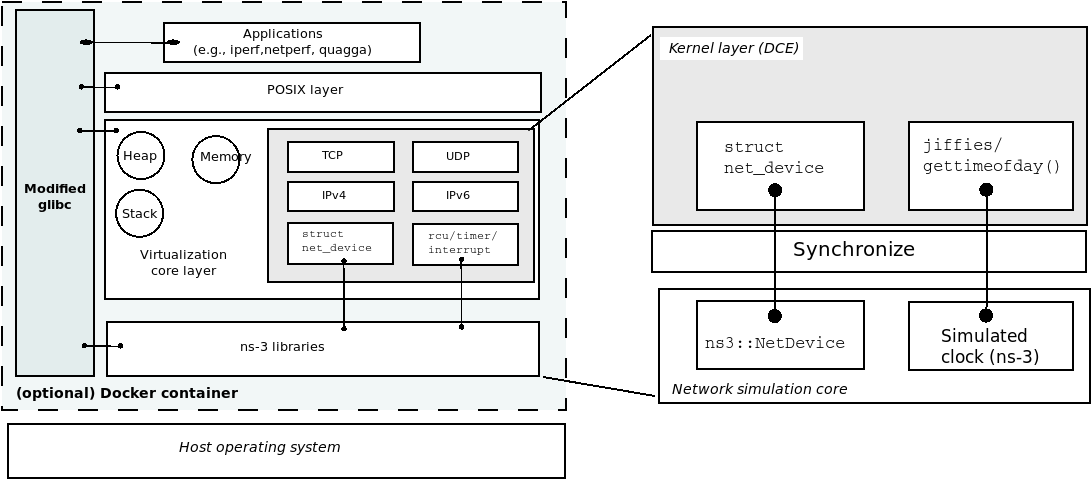
\includegraphics[width=0.95\textwidth]{figs/architecture.png}

  \caption{DCE architecture (redrawn from Figure 1 of [1]) with recent extensions highlighted}
  \label{fig:architecture}
\end{figure*}

Figure \ref{fig:architecture} provides an architectural overview of DCE;
this figure is partially redrawn from a similar Figure 1 of \cite{Tazaki13},
with extensions to highlight the contributions reported on herein.
In the lower center are ns-3 libraries; these libraries, along with simulation
programs that link to them, are the typical ns-3 simulation components.
Sitting above ns-3, in this diagram, is DCE.  DCE provides additional
libraries that can be used in place of ns-3 libraries, at the TCP/IP and
application layers.  The box bounding TCP, UDP, IPv4, and IPv6 depicts 
how the Linux (or FreeBSD) kernel is itself built as a library.  Data
packets flow across the boundary between a Linux struct net\_device and
the ns-3 NetDevice object, and additional system support, such as providing
time routines to kernel code, is synchronized with the ns-3 core.
The DCE virtualization core layer manages resources for the various DCE
applications, including file system access, heap- and stack-allocated
memory, global variable handling, and thread management.
Above the (optional) DCE kernel library is a POSIX interface layer that
DCE applications link to.  This layer redirects system calls, such as a
call to open a socket, to ns-3 or the DCE kernel; in essence, it reimplements
and redirects parts of the C standard library.  DCE applications are compiled
and linked with a few extra arguments such that they are built as 
position-independent executables (PIE), and a special DCE Executable and
Linkable Format (ELF) program loader
ensures that all of the application's symbols can be loaded multiple times
(as needed) into the ns-3 address space.

\sloppy DCE is a sophisticated piece of software, and after an intensive period
of development and initial releases, the maintenance of DCE has been
semi-dormant for the past five years or so.  As a result, the host
operating systems that DCE is compatible with are stuck in the past.
The most recent Linux distribution compatible with the latest (DCE-1.11)
release is Ubuntu 16.04.  It has been estimated
\footnote{\url{https://www.theregister.com/2020/01/06/linux\_2020\_kernel\_systemd\_code}}
 that, in 2020, roughly 27.8 million lines of code were added to Linux
kernel and systemd, with roughly 75,000-80,000 commits per year. Although
DCE does not have to change for most of these commits, it should be clear
that the host operating system environment that DCE has to live within
undergoes rapid change, leading to a DCE maintenance burden.

This paper reports on a recent project to restore DCE's compatibility with
recent Linux releases and kernel stack versions.  The project required
a lot of adjustments to DCE to account for changes in Linux and in the
C (and C++) standard library (on Linux, this library is called \emph{glibc}).
Figure \ref{fig:architecture} highlights one of the outcomes; the need to
include a modified, custom version of the glibc standard library.  To
simplify the installation burden on users, we also developed a Docker
container framework with a pre-built modified glibc.  The reasons for
doing so are described in Sections 2 and 3.  Finally, we updated the
version of the Linux kernel library for DCE from kernel version 4.4 
to kernel version 5.10.  A new DCE release (1.12) is being prepared with
capability to run on Ubuntu 20.04, and the use of Docker will facilitate
use on other modern Linux systems as well.

The rest of this paper is organized as follows:
\begin{itemize}
\item Section 2 provides an overview on the technical challenges due to Linux and glibc evolution.
\item Section 3 outlines our solutions to these challenges.
\item Section 4 presents a performance evaluation of the new software.
\item Section 5 describes related work.
\item Section 6 covers our conclusions and directions for future work.
\end{itemize}

\section{Challenges}

\subsection{libio vtable mangling}
DCE requires to map FILE operations to it's internal custom handlers which work in synchronization with ns-3. DCE supports different operations on a FILE 
through a Unix file abstraction, which requires all FILE operation calls to be mapped through it. This requires us to modify the vtable entries for the FILE
object accordingly.

The vtable is a table maintaining references to functions called for virtual functions defined for a class or an entity and changes dynamically 
during runtime unlike compile time decisive function calls. The FILE structure is a library defined structure which defines the overall organization, 
orientation and properties of any file I/O stream opened
by the host application. It maintains different parameters for storing useful operational fields like the UNIX based file descriptor number of the 
opened stream, the read/write offsets and buffer addresses of the stream. The pseudoname for the FILE structure as seen inside libc is \textit{\_IO\_FILE}. 
Since, FILE is a library defined entity, the library provides its own set of implementation for all possible operations on an open FILE stream.
Whenever an \textit{\_IO\_FILE} stream is allocated by the kernel, a contiguous memory location is allocated as a block called \textit{\_IO\_FILE\_plus}. 
The \textit{\_IO\_FILE\_plus} structure looks like this.

\begin{lstlisting}[style=CStyle]     
struct _IO_FILE_plus
{
  FILE file;
  const struct _IO_jump_t *vtable;
};
\end{lstlisting}

By nature of the implementation of the kernel's memory allocation processes, the contents of a struct are allocated in contiguous memoory locations. 
The FILE and the \textit{\_IO\_jump\_t} objects are allocated in contiguous memory locations. Specifically, the 
\textit{\_IO\_jump\_t} areas is interesting to DCE, as it defines the callbacks or reference pointers to the functions handlers for each supported file 
operations such as , texttt{read}, \texttt{close}, \texttt{seek}, \texttt{write} and \texttt{stat}.

This structure acts like the vtable for the FILE structure, but it does not behave like the oridinary vtable seen when working with virtual functions 
and derived classes, which are dynamic and supports run time bindings. This vtable is instead expected to behave as a statically bound vtable.  There exist 
other libc functions, like \textit{fopencookie}, to override some of the FILE operation implementations, but not all operations are supported, and 
\textit{fopencookie} also does not attach itself to a standard file I/O stream, 
instead works  with user defined buffers a.k.a cookies. 

Taking advantage of the contiguous memory allocation of the FILE and \textit{\_IO\_jump\_t}, one can overwrite the vtable with a custom vtable definition for all
the operations needed for DCE. One can make a dummy \textit{\_IO\_FILE\_plus} 
pointer point to the explicitly casted FILE object. \textit{memcpy} the existing vtable to a local copy, modify and overwrite the stream operations with
custom written function pointers, and then re-point the vtable field of the dummy \textit{\_IO\_FILE\_plus} to the local modified vtable.  This allows
control over stream operations, which can now be routed through DCE and made to behave as ns-3 streams, Unix FD streams, etc. based on the type of file 
descriptor that is defined.

\sloppy Post libc-2.25, security features have been implemented to glibc to identify 
and prevent such block buffer overflow attacks on the FILE object. Whenever any FILE
operation is executed, glibc 
verifies the FILE object's vtable. It makes a call to 
\textit{\_IO\_validate\_vtable}. Every libio vtable is defined in a unique section called \textit{libio\_IO\_vtables}. By definition, libc trusts
the vtable if the vtable of the current FILE object lies within this section. It checks if the offsets of this vtable lies between 
\textit{\_\_stop\_\_\_libc\_IO\_vtables} and \textit{\_\_start\_\_\_libc\_IO\_vtables}, if it does, we can continue with the operation, if not, libc 
conducts a final check by calling \textit{\_IO\_vtable\_check} which makes final checks on the FILE vtable pointer location, namespace and edge cases
where FILE * objects are passed to threads which are not in the currently linked executable.  When DCE overflows the \textit{\_IO\_FILE\_plus} and 
overwrites the \textit{\_IO\_jump\_t}, it does not lie in \textit{libio\_IO\_vtables} section and it also does not pass the pointer mangling sanity checks, leading to 
a \textit{Fatal error: glibc detected an invalid stdio handle}

\subsection{PIE loading and usage}
Position-independent-executables (PIE) are applications compiled with special compiler flags that allow the application to be loaded into an arbitrary
memory address, not depending on absolute symbol addresses. DCE needs to have position independent executables, so that when they are loaded into memory,
the symbol positions in memory are dynamic, giving control over when the application main is called in a simulation.To implement this, DCE uses the \textit{CoojaLoader}
which uses \textit{dlmopen} under the hood to load the executable into memory. In glibc library versions newer than 2.25, security checks have been introduced to 
identify such PIE objects being loaded through \textit{dlmopen}, and in case the \texttt{DF\_1\_PIE} flag is found in the object's ELF Dynamic headers, it will abort 
with an error.
 

\subsection{Linux Networking Stack for DCE}
A Linux kernel library port allows DCE to export callback structures, abstracting the internal network data flow, coordinating Linux kernel synchronization, 
process creation, and DCE-kernel task, IRQ and tasklet scheduling and synchronization, to expose a Linux-like execution environment for host applications. 

Two potential projects or architectures to implement this are LKL and LibOS, which are discussed next.

\subsubsection{LKL}
The Linux Kernel Library (LKL) is a library port of the Linux kernel that, through some pre-shipped helper shell scripts, can be used to hijack
all system calls made by a host application and map them through the ported Linux kernel rather than through system defined implementations. It also allows one 
to setup network interfaces such as TAP, RAW, VDE , etc. with custom gateways, netmasks, IP addresses, etc. with the help of JSON configuration files. These helper
shell scripts make use of \texttt{LD\_PRELOAD} to reorder library loading to LKL written system calls to take control in place of the libc defined routines.
 
\subsubsection{LibOS}
LibOS uses the same internal architecture as does \textit{net-next-nuse}.
It is also a Linux kernel port that works on the principle of selective 
kernel module linking and patching. It defines special link time constructs
to include only specific kernel files and 
symbols that are needed for executing on top of the Linux kernel with \textit{nuse}, which works similar to LKL by hijacking system calls 
and rerouting them through nuse and kernel defined routines.

\subsubsection{LKL vs. LibOS}
We conducted a comparison of LKL and LibOS approaches according to different design parameters and considerations for a complex application framework such as
DCE with very specific demands from it's underying network stack.

\paragraph{Linux feature support \& Maintenance}
On comparing LKL with LibOS, on the ease of entending support for Linux features which are compiled into the shared library port and 
can be used through the API, LKL seems to win here, as adding support for new features in later kernels can be as easy as a git rebase, as not kernel internal code  
is manipulated and also the Kernel is built using minimal changes to the original Linux build steps. net-next-nuse on the other hand, would require selective Linux 
kernel linking, bridges the gap between application workspace and Linux kernel networking stack with the help of glue code, kernel component connector code, and user 
application provided exported functions and callbacks for proper execution, which increases maintenance cost.

\paragraph{Library kernel boot order and scheduling}
Both LKL and LibOS differ form each other on how it initializes the kernel and schedules tasks, which also determines many execution factors of DCE. 

LKL spins up a high level CPU lock controlled thread, which makes calls to \texttt{start\_kernel}. Since LKL is a uniprocessor system, it initializes 
the kernel on a singular LKL thread, 
locks of which are synchronized with Linux scheduler calls, which are called when the scheduler decides to switch execution control 
to kernel level tasks for preemption, and other tasks, which require certain memory level moderation to achieve
atomic operation. Since, the LKL thread can only be preempted by kernel level tasks and not through LKL API, launching a second user task is not possible if 
CPU lock is held, blocking the DCE script execution infinitely which works based on LWPs.

LibOS makes 
use of its own \texttt{lib\_init} fuction which calls specific setups calls required to initialize the kernel.
It also overrides scheduler member functions, syncing it with ns-3's 
scheduler. LibOS creates an ns-3 task copy for each kernel task which is created by the \texttt{copy\_process}, \texttt{create\_process},
etc. Each such task maps with itself a callback function which should be called once the wait time
for a task is over, or has been invoked as a part of a regular scheduling process. Once tasks are processed, they are 
also popped off the ns-3 task queue.

\section{Solutions}
\label{section:design}

\subsection{Custom glibc-2.31-based build}
The section discusses how the modified glibc is patched to disable problematic security checks which were discussed as some of the challenges previously
in the paper and also explains how the link procedure works.

The DCE script \texttt{dcemakeversion.c} help generate .version files for all the system shared library which are statically linked to DCE's custom libc. A 
shared library \texttt{libc-ns3.so} is created with symbols tagged as NATIVE and DCE based on there position of declaration which are mapped through the 
\texttt{libc\_setup} function. The DCE type symbols are implemented 
inside the DCE source code. Users compile their applications with an extra -fPIC and -pie flag, which helps DCE load the applications dynamically into the DCE process 
address space. The main of these application are then called based on the simulation script, which if require FILE operations would require DCE to To override the vtable 
mangling security checks of glibc, 
for which it is necessary to override the security checks on vtable pointer mangling. A security patched glibc is build and installed on a specific location. gcc is then made 
to use that directory as the SYSROOT and also point the library, header and ELF executable lookup directories to our custom glibc using -L, -I, --rpath and --rpath-link.


\subsection{Bake Build Automation}

The process of the modified glibc and Linux compilation can be automated using Bake.
Bake has a source configuration option named \textit{patch}, which can safely apply a patch, without re-applying if it has already been applied before.  
This allows, for example, a large codebase to be fetched in its unaltered form, while Bake must maintain and apply only a small patch file to it.
Using this option, Bake applies the DCE-specific glibc patch, which disables the security checks on vtable mangling, and also disables the 
PIE object checks for dlmopen position independent executable loading. The glibc is then build using its standard build steps. The linux kernel headers
files are then installed into the \texttt{/usr} directory of a custom glibc's sysroot. This finishes with a standard Linux-like system root to use for building 
DCE without any issues. 


\subsection{Docker environnment for DCE}
DCE has a long dependency graph which includes dependencies across 
system libraries, other projects, Linux kernel and tools, host specific requirements, etc. To ease installation process and standardize the process 
across docker supported Linux distros, a docker based setup is discussed.


\begin{figure}[!htb]
  \centering
    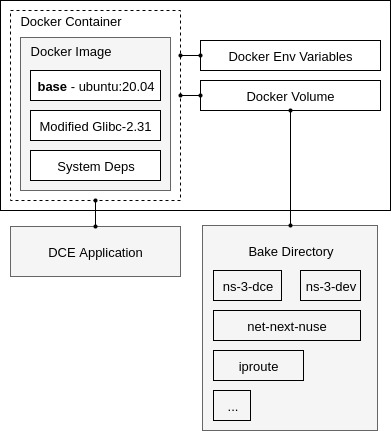
\includegraphics[width=0.30\textwidth]{figs/docker-architecture.jpg}

  \caption{DCE docker architecture composition}
  \label{fig:docker}
\end{figure}


The docker release consists of the above docker network setup which is orchestrated using a Docker Compose script. 
It consists of the docker container, environemnt variables and Volume. The docker 
container works on a custom image which uses ubuntu:20.04 as the base image. A docker image is collection of Image Layers. Each image layer is a 
Dockerfile command which adds up to create the final docker environemnt for that image. The docker image has been optimized to use minimal number of layers and 
all redundant layers are merged together. A layer for installing all system dependencies and libraries ensures all listed and unlisted bake 
dependencies for building DCE are satisfied. It also has a pre-compiled glibc bundled into the image itself. This helps us reduce the docker 
image size drastically as compared to the building from source everytime which might consume GBs, but this layer takes up 51.36 MB.
It also has a default environemnt variable 
\texttt{DCE\_WITH\_DOCKER=1} which is a flag variable for ns-3-dce waf script to try and execute a docker based build.

The container, as dicussed before, comes with a pre-compiled glibc-2.31 and so the user does not need to build the modified glibc again from source.
The environment variable \texttt{DCE\_WITH\_GLIBC} tells waf where to look for the modified glibc build directory. This environemnt variable can 
later be changed from inside the docker container to point to a custom glibc build directory if the user wishes to do so. This glibc build is then 
used by the ns-3-dce waf to compile ns-3-dce. The docker compose also sets up a volume. A docker volume is a mechanism which lets docker containers 
use persisting data from within the container. Docker containers can attach volumes to themselves
and map specific directories from withing the docker container to the host directory. Any changes made to that directory withing the  docker container
is visible and persisted on the mapped host directory and also vice-vers. This is a key requirement for us, as ns-3 projects are used by both 
researchers and users who wish to just simulate scripts and also project maintainers, contributors and testers who need to be able to make changes 
to the ns-3 code locally using text editors and IDEs, and test it instantly, also access simulation output files on local file explorer and 
third party applications. So, we attach a volume which maps the /home/bake directory from within the docker container to the bake directory on 
the host.

The ns-3-dce waf script supports both docker based build and native builds on the same branch. It selects the glibc 
build directory based on waf configure and local environemnt variables and compiles ns-3-dce on top of it.


\subsection{net-next-nuse-5.10}
Net-next-nuse, introduced above, is an architecture port of the Linux kernel, which resorts to selective kernel module linking and which takes control over 
critical kernel 
components such as memory SLAB allocators through internal DCE callbacks mapped to internal SLIB interface, 
task schedulers and timer functions, provided Linux network stack as library through an exported API.

\subsubsection{Background}
In this section, we will see what are some of the major challenges which net-next-nuse solves and the basics of how the Linux kernel is modified to 
accomodate this type of architecture.

Net-next-nuse understands that the way Linux Kernel behaves on the host, and the way the kernel interacts with the task 
scheduler and how the scheduler operates on the tasks, is completely different from how DCE manages fibers (called tasks in DCE terminology). 
DCE is based on context-based, lightweight threads called fibers, which require a custom scheduler, called the TaskManager in DCE. On an ordinary
host machine, when a user runs any application that spins up normal threads, , making the kernel responsible for jumping from one thread to another. 

Net-next-nuse uses fibres, which lets one jump from one thread to another only when one of the fibers yields to another fiber, and this context switch 
is done by a custom scheduler, which is written in DCE's TaskManager::Schedule(). This is beneficial because when using ordinary threads, 
the number of context switches the CPU has to do (push your thread data stack on to you address space, in and out), 
is a lot more expensive than making switches in fibers. This also eliminates the dependence of the kernel to bother about scheduling the threads on 
the different cores of the host CPU and maintaining mutex locks of the CPU inside the kernel library. To manage the isolated kernel threads inside the library , 
net-next-nuse  performs  a selective linking of 
kernel modules and utilities and to avoid linking the scheduler, workqueue, waitqueue and other such linked components, opting to instead implement
them using DCE imported functions mapped to TaskManager utilities. As a result, every time that some process wants to preempt and block, the kernel calls 
\texttt{schedule()} or \texttt{schedule\_timeout()}, and control is passed to DCE to take care of it. 

\subsubsection{Virtual Kernel Task and its Real Fiber Equivalent}
net-next-nuse uses exported functions and internal DCE calls to allow kernel task creation  which are exposes to net-next-nuse through an API during library object.
initialization.

\sloppy Every new task inside the kernel, for example, a syscall, 
creates an internal kernel thread.  When a system boots up, there has to be some initial task that invokes the \texttt{start\_kernel(...)} 
function. This is called the \texttt{init\_task}. Whenever a new kernel thread is to be created, a call to \texttt{kernel\_thread(...)} is made. Along with the 
function that is to be invoked in the thread, and the arguments to be passed, one must also pass along one more argument, known as clone flags. 
Internally, the kernel will try to clone a previous task as much as possible. These flags basically determine 
how far the kernel should go, as in cloning the structures. Some of the flags are \texttt{CLONE\_FS}, \texttt{CLONE\_VM}, \texttt{CLONE\_FILES}, etc., 
and \texttt{kernel\_clone(...)} passes a special clone flags data structure. This function further calls \texttt{copy\_process(...)}, which is responsible for checking 
which flags are enabled using a bitwise \texttt{\&} operator and calling the corresponding copy utility; for example, \texttt{copy\_fs(...)}, \texttt{copy\_files(...)}, 
and \texttt{copy\_cred(...)}.  It also makes a call to \texttt{dup\_task\_struct(...)}, which will bind changes of the current \texttt{task\_struct} to a new one and 
return it back. After receiving back a proper \texttt{task\_struct}, the \texttt{kernel\_clone(...)} schedules a fork for the newly created task.

\sloppy Therefore, to take  control over the kernel thread creation, we rewrite the \texttt{kernel\_thread(...)} function to call 
\texttt{lib\_task\_start(...)}, which calls the 
internal TaskManager::Start(...) to create a DCE task, fills up the task\_struct, sets the SimTask context with the task\_struct and returns back 
the process ID (pid) of the task. Also, \texttt{current}, as previously referred to above, is not a variable, but a macro, which calls \texttt{get\_current(...)}, which DCE hijacks and leads to TaskManager::TaskCurrent(...), which checks if the current task has a SimTask context. If it does, it returns it back. 
If it does not, it calls TaskManager::Start(...) to set it up and every time 
TaskManager::TaskWait(...)  is called on a particular task, DCE can put the current job to sleep, and give the other tasks/fibers a chance to 
execute their set of functions. 
 
\subsubsection{Kernel initialization}
The kernel initializers are divided into base init functions and roughly eight levels/types of initcalls, and export a start and end pointer of the list of initcall list. 
The initcalls are stored in a special .initcall.init section of the final linked library, which are then copied to their respective positions through the linker.lds script.
Some of the new additions made to original initcall list are : 

\begin{itemize}
  \item vfs\_caches\_init\_early : To allow mounting of file systems such as \texttt{/proc} and file operations, which require the linked lists for 
  dcache(Directory Entry Cache, which helps fast lookup of recent paths) and inode.
  \item cred\_init : Steps up the \texttt{creds\_jar} cache which is required by the LSM \hyperref[Section_LSM]{3.4.7}, fs module and 
  while creds initialization for kernel task creation.
  \item proc\_root\_init : Sets up the \texttt{/proc} filesystem root cache, symlinks for mounts, net namespace for proc, and required directories.
\end{itemize}

The initcall invocation loop of lib\_init was also changed to use \texttt{initcall\_from\_entry} instead of a direct function call. 
This invocation function does a safe offset based function address lookup and calls the init method accordingly. 
Before we call all the init functions, I also initialized the \texttt{files} and \texttt{fs} cache pointers for cache based memory 
allocation using \texttt{kmem} in file operation methods, with slab objects aligned to a cache line, panic enabled on relocation errors, and also accounting enabled 
for the cache. These caches are required while setting up the \texttt{fs\_struct} and \texttt{files\_struct} for each new task in its 
corresponding \texttt{task\_struct}. 

\subsubsection{Security LSM Module}\label{Section_LSM}
Certain kernel initialization procedures proceed only when the desired actions are allowed by the LSM. Below is a brief description of why the LSM is requied and how 
it is included into net-next-nuse.

In newer Linux releases \texttt{vfs\_kern\_mount(...)} validates the file system mount context and parses params using \texttt{security\_fs\_context\_parse\_param(...)},
which checks if the requested operation was blocked in the LSM tables. If this module is not enabled, it would return back ENOPARAM by default and fail. This makes it 
important for us to link the LSM, and setup our build/linking scipts accordingly.

The security module of the Linux kernel depends on a special configuration called the \texttt{CONFIG\_LSM}. The LSM module requires a few architecture
defined variables, which are placed in a specific section
of the library called .init.data section using the \texttt{AT(ADDR(...))} directive, through linker script. 
The below code keeps sections \texttt{lsm\_info.init} and \texttt{early\_lsm\_info.init} even if not referenced using the \texttt{KEEP} directive , 
and also defines start and end information sections of both.  The implementation of them were drawn from LKL's LSM definition.

\subsubsection{Kernel code and net-next-nuse alignment}
When net-next-nuse is loaded as a shared library into DCE and \texttt{lib\_init(...)} is called, it invokes certain kernel methods, which triggers 
kernel initialization routines which help setup critical components such as the mount namespaces, vfs, kernel threads and tasks, etc. 
Since Linux kernel 4.4.0, the
kernel has envolevd a lot in terms of how the kernel gets initialized. The section below discusses some of the alignments which had to be made with respect to 
Linux kernel 5.10 to integrate net-next-nuse's architecture.

The kernel depends on certain namespace based constaint variables while initializing the kernel. One such requirement is the \texttt{UCOUNT\_MNT\_NAMESPACES}
of the \texttt{init\_task}. Since a complete architecture port is not needed, this value is not defined, so atomic reads on this value would seg fault. So 
we manually set it to \texttt{MNS\_MAX} for the current task's nsproxy. One other alignment was the \texttt{sock\_init}, which is dependent on the proc file system  
to setup the sysctl interface using \texttt{net\_sysctl\_init(...)}. Then the sockfs filesystem is registered using \texttt{register\_filesystem(...)}. Previously,
sockfs file system init did not depend on a file system context and required only a mount function \texttt{sockfs\_mount}, but in a later Linux commit the sockfs 
mounting process was handed over to the internal VFS mounting initcall, thus we had to glue code the \texttt{mnt\_init(...)} initcall. Many other alignments, such as,
atomic operations, NAPI atomic read issues, etc. were fixed based on later Linux commits which were introduced.

\iffalse
\subsubsection{Native Kernel NetDevices}
Certain components of ns-3 require the setup of custom NetDevices which require a custom MTU and other flags, such as whether the device should enable multicast, 
or is it a point-to-point device, etc. These flags can be put together, and one can allocate a Linux netdevice struct for each such requirement using
the \texttt{alloc\_netdev(...)}, passing all of the configuration needed for details such as MTU, address length, and destructors, along with 
a \texttt{register\_netdev(...)} call.
This returns back a forward declared struct SimDevice which is used as a NetDevice object inside ns-3 which is required by ns-3's core networking modules.
\fi

\section{Performance Evaluation}
We describe some performance evaluations of the DCE code, following the
approach described in \cite{Tazaki13}.  The purpose of this section is to
compare the runtime performance of different versions of DCE and different
DCE configurations with the performance reported in \cite{Tazaki13} and with
a equivalent ns-3 (without DCE) simulation.

\begin{figure}[h!]
  \centering
    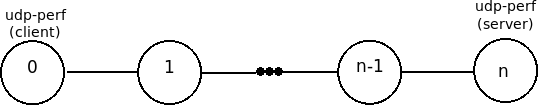
\includegraphics[width=0.47\textwidth]{figs/topology.png}
  \caption{Simulation topology (redrawn from Figure 2 of \cite{Tazaki13})}
  \label{fig:topology}
\end{figure}

The simulation topology used is shown in Figure \ref{fig:topology}, which
is duplicated from Figure 2 of \cite{Tazaki13}.  The topology is a simple
linear network with a variable number of hops, and a single UDP flow
is sent from client to server for the duration of the simulation.
The UDP data rate is configurable between 5 and 100 Mbps, and the UDP
payload size was a uniform 1470 bytes per packet.
To avoid per-hop congestion, link bandwidths are set to 1 Gbps.
For the purpose of runtime performance comparison, this topology is
suitable because it makes use of a DCE application (a custom UDP traffic
generator (\emph{udp-perf}) written in C and maintained as part of DCE),
and allows the enabling or disabling of kernel-mode operation.  Most
simulation operations involve the creation and transmission of packets.
The program to realize this topology is found as an example named
\emph{dce-udp-perf.cc} in the DCE codebase; we only had to make minor
updates to that program to realize the different configurations reported
herein, and we believe that this is the program originally used
in \cite{Tazaki13}.

We do not know what version of DCE was used in \cite{Tazaki13} but we
have reason to believe that it was not significantly different from the
most recent DCE 1.11 release of DCE (for Ubuntu 16.04), because there
has not been much development of DCE since the publication of \cite{Tazaki13}.
The new software we are reporting on herein (for Ubuntu 20.04, with newer
kernel code, and optionally with Docker) will be part of DCE 1.12 and
later releases.

ns-3 and DCE software can be compiled in debug or optimized mode.  For
these experiments, we compiled both ns-3 and DCE in optimized mode.  All
other software (e.g. net-next-nuse-4.4.0, glibc-2.31) was compiled in
the default mode specified for that software.

For the experiments, we used two different machines (for the two different
operating systems).  As DCE execution time is dominated by the single thread
CPU performance of a machine, execution of the same program on different CPUs
will lead to
different runtimes.  In \cite{Tazaki13}, an Intel Xeon 2.8 GHz machine was
used; this CPU is rated with a single thread performance of 384 by PassMark
Software's online CPU benchmark dataset\footnote{https://www.cpubenchmark.net}.
We used an Intel Core i7-4770 3.40 GHz machine for tests of DCE version 1.11
on Ubuntu 16.  This CPU has a single thread benchmark of 2167 according
to the same database.  For tests of DCE version 1.12 (Ubuntu 20.04), we used
a machine with an Intel Core i7-1065G7 1.30 GHz CPU.  This CPU has a
single thread benchmark of 2416 according to the same database.  Use of
different machines for the two different operating systems makes it difficult
to directly compare the DCE performance results, but because we are able to
run the same ns-3 simulation on both machines, we can calibrate the
performance by referencing DCE performance results in relation to the
corresponding ns-3 runtimes on each machine.

\begin{figure}[h!]
  \centering
    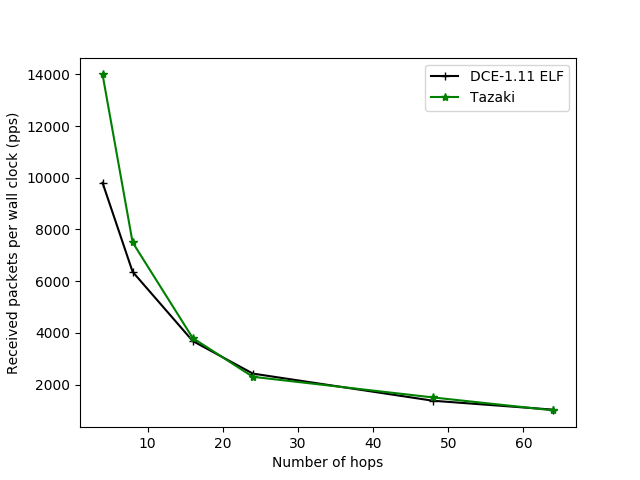
\includegraphics[width=0.47\textwidth]{figs/hops-vs-pps.png}
  \caption{Packet processing performance as a function of number of network hops}
  \label{fig:hops-vs-pps}
\end{figure}

Figure \ref{fig:hops-vs-pps} reproduces data from a similar figure (Figure 3)
in \cite{Tazaki13}, and provides some new data for current simulation runs.
In \cite{Tazaki13}, this figure was used to compare performance between
DCE and Mininet-HiFi.  Here, we compare the previous data on DCE from
\cite{Tazaki13} (read from the paper figure) with a similar experiment run
with DCE version 1.11 on Ubuntu 16.  A single simulation trial for different
values of network hops (4, 8, 16, 24, 48, 64) was run for 50 simulated
seconds, and the number of received packets was divided by the elapsed
wall clock time of each trial, to yield a packets-per-second measurement.
This experiment illustrates that the most recent release of DCE code has a
similar performance profile as that of \cite{Tazaki13}.  Because the
number of packets sent in each simulation is the same, the downward
slope of the curves as the number of hops increases indicates that larger
topologies (which cause more simulation events to be generated per packet)
will run more slowly.  We also note that an unexpected result of this
experiment was that the two curves would generally overlap, since the
simulations were conducted on machines with different CPU performance.
This could indicate a performance regression between the version of DCE
used in \cite{Tazaki13} and the most recent release; performance regression
has not been tracked as part of DCE maintenance.

\begin{figure}[h!]
  \centering
    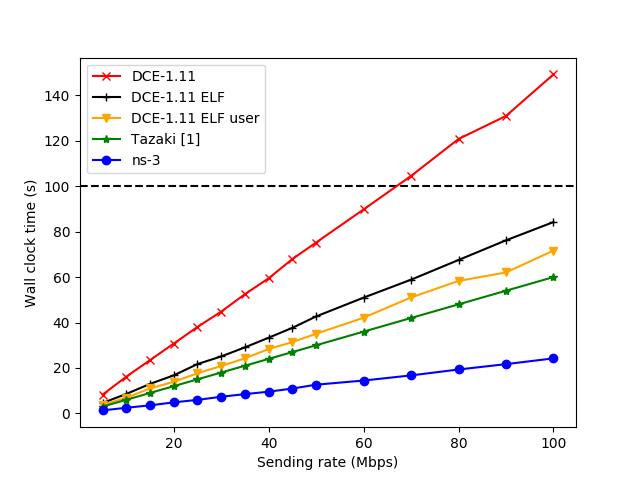
\includegraphics[width=0.47\textwidth]{figs/rate-vs-time.png}
  \caption{Sending rate vs. wall clock time on a four hop topology for different DCE configurations (Ubuntu 16)}
  \label{fig:rate-vs-time}
\end{figure}

Figure \ref{fig:rate-vs-time} recreates a similar experiment 
(shown in Figure 5 of \cite{Tazaki13}) to highlight the impact of sending
rate on the wall clock time of the simulation trial, for different sending
rates on a four-hop topology.  As in \cite{Tazaki13}, a linear relationship
between the sending rate and wall clock time is expected, because the
number of hops per packet is held constant.  Again, we reproduce the
curve from \cite{Tazaki13} by reading their data from the paper figure.
There are several interesting observations.  First, we believe that the
closest comparison between the experiment from \cite{Tazaki13} is the
\emph{DCE 1.11 ELF} result.  This configuration used DCE with Linux kernel
version 4.4.0 and the ELF loader (known to lead to faster simulation
runs than the default Cooja loader).  Despite executing on a much faster
machine, the DCE 1.11 result is slower than the earlier reported simulation.
Again, we do not have specific information on how the previous run
was conducted (the website hosting the scripts is no longer active), and
it could possibly be due to performance regressions either with DCE
or with the Linux kernel library (\cite{Tazaki13} used a virtualized kernel
version of 2.6.36).  Aside from this difference, this figure can be used
to compare the execution time performance of different modes of DCE.
For comparison, we added a mode of operation to \emph{dce-udp-perf.cc} to
bypass the use of the \emph{udp-perf} DCE application and to use the
ns-3 UDP client application.  The blue line (bottom) is therefore a pure
ns-3 simulation, and runs fastest.  The next fastest execution is found
with \emph{DCE 1.11 ELF user}, which is using the ELF loader with DCE
running in user-mode, not kernel-mode.  This means that the DCE application
is using the ns-3 TCP/IP stack rather than the Linux kernel stack.  The
next fastest configuration is the \emph{DCE 1.11 ELF} configuration, using
DCE user-space and kernel code over the ns-3 simulated point-to-point links.
The final curve is the \emph{DCE 1.11} curve that uses the DCE user-space
and kernel code but with the default Cooja loader.  This curve shows that
the use of the ELF loader conveys a significant performance benefit.
While the Figure 5 of \cite{Tazaki13} includes plots for other network
diameters (up to 32 hops), we omit the larger topologies in our figure
for clarity; the larger topologies display similar linear relationships.
The horizontal dashed line depicted shows the performance point at which
the simulation time equals the wall clock time; only the DCE 1.11 curve
for data rates greater than 60 Mbps ran more slowly than real time in
these experiments.

\begin{figure}[h!]
  \centering
    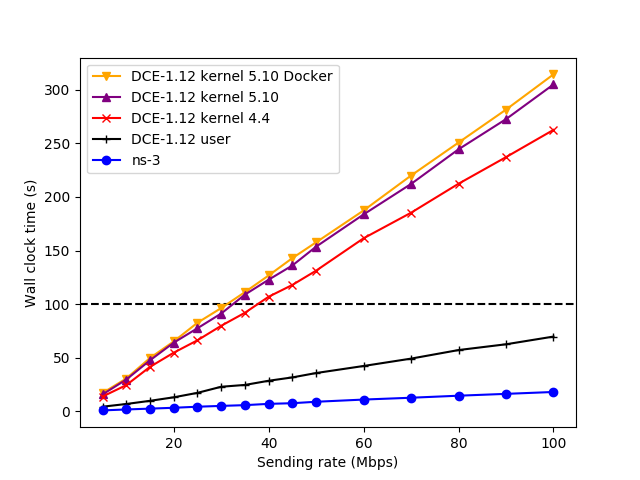
\includegraphics[width=0.47\textwidth]{figs/rate-vs-time-dce12.png}
  \caption{Sending rate vs. wall clock time on a four hop topology for different DCE configurations (Ubuntu 20)}
  \label{fig:rate-vs-time-u20}
\end{figure}

Figure \ref{fig:rate-vs-time-u20} presents comparable simulation results
for the new version of DCE (the pending 1.12 and later releases).  As noted
above, the machine for these experiments had a faster CPU, and in comparing
the pure ns-3 results between both machines, the simulation runs on this
machine were about 25\% faster (although the ns-3 versions were different,
ns-3.34 on DCE 1.11 and ns-3.35 on DCE 1.12, this is not expected to
lead to any notable difference in performance).  The next curve above
the ns-3 curve, \emph{DCE-1.12 user}, can be compared with the
\emph{DCE-1.11 ELF user} in the previous figure.  In Ubuntu 20.04, the
ELF loader is not yet working, so the comparison is not exact, but the
experiment shows that despite the lack of ELF loader, use of the ns-3
stack in both cases leads to faster than real-time execution.

Next, compare the red curves, \emph{DCE-1.11} vs. \emph{DCE-1.12 kernel 4.4}.
Neither configuration used the ELF loader, and both used the same Linux
kernel library version (4.4).  However, the DCE-1.12 version uses the
modified glibc library.  The newer DCE version results in 75\% more runtime
despite being on the faster machine.  

The final two curves illustrate performance differences between the current
kernel library version 4.4 and a new kernel library (5.10), and the
difference between running DCE natively on the host operating system vs.
running within a Docker container.  The newer kernel library required
about 16\% more runtime.   Running within a Docker container was observed
to incur only about a 3\% performance hit.

As of this writing, the performance differences between the newer DCE 1.12
versions and the last released (DCE 1.11) versions have not been debugged
or profiled; the differences were discovered during the course of preparing
this paper.  The small performance cost of running within a Docker container,
however, may be worth the convenience to future users.

\section{Related Work}
We do not provide a lengthy list of other simulation frameworks related
to DCE, or other different approaches to mixing implementation code with
simulations; the interested reader is directed to \cite{Tazaki13} and
\cite{Lacage10} for such references.  We focus here on related work that has
been published since \cite{Tazaki13} was published in 2013.

We are not aware of anything comparable to DCE having been published in
the past eight years, either for ns-3 or for other system simulators.  
During that time period, more attention has been paid on the use of
ns-3 emulation features or on container-based network experimentation
frameworks such as Mininet \cite{Handigol12}; a recent tool in this regard is
NeST \cite{Rai20}.  One of the most similar approaches to DCE appears to
be the Open Network Emulator (ONE)\cite{Duggirala12}, which leverages the
Clang/LLVM
toolchain to convert applications to modules that can be integrated
with a network simulation stack.  The NCTUns simulator \cite{Wang03}
is a commercial simulator that advertises a 'kernel-reentrant' mode
of supporting Linux network stack code in a simulation.  Both of these
tools were developed during the same timeframe as DCE.

There also appears to be very little published regarding the extension
of DCE or analyses of its performance.  The work by Ivey \cite{Ivey16}
describes an extension of DCE to support not only C and C++ but also
Python- and Java-based programs.  The main interest in doing so was
to enable DCE use of software-defined networking (SDN) applications,
many of which are implemented in Python or Java.  However, these
extensions appear to never have been publicly released.  
One paper published about five years ago \cite{Wiggins16} began to explore
a possible performance bottleneck arising from how DCE makes use of multiple
cores to distribute processes onto different threads, and speculates that
cache consistency overhead may account for the observed counter-intuitive
result that a DCE experiment may run significantly faster on a single core
machine than on a multi-core machine.   Further profiling of our performance
results in this regard is definitely warranted. 

\section{Conclusions}
%\end{document}  % This is where a 'short' article might terminate
The paper discusses the way DCE was modernized to work on newer Linux environments, 
use newer Linux networking stack and kernel and also compares against other alternatives. 
It also suggests ways to improve project deployment using docker and compares performance results across different platforms and stacks.

The next step would be to profile DCE further to understand what are the other parameters which determine 
the runtime of scripts. We also plan to work on building a more modular Linux library port with an efficient 
middleware notification based task synchronizer, which would have less maintenance cost and increased kernel feature availability.
 We also plan to work on Ipv6 support for net-next-nuse-5.10 on the same architecture as now. Building an elf-loader for the libc-2.31 will also be a 
 suggested future effort, as it reduces DCE execution time drastically.

%ACKNOWLEDGMENTS are optional
\section{Acknowledgments}
This project was funded by the 2021 Google Summer of Code.
%
% The following two commands are all you need in the
% initial runs of your .tex file to
% produce the bibliography for the citations in your paper.
\bibliographystyle{abbrv}
\bibliography{revitalizing-dce}  % sigproc.bib is the name of the Bibliography in this case
% You must have a proper ".bib" file
%  and remember to run:
% latex bibtex latex latex
% to resolve all references
%
% ACM needs 'a single self-contained file'!
%
%APPENDICES are optional
%\balancecolumns
%\balancecolumns % GM June 2007
% That's all folks!
\end{document}
